\chapter{测试时适应}

\section{Cross-Domain FSCIL：从类别变化到数据分布变化}

在《DML：为什么模型的置信度不等于模型对世界的认识程度？》《DPM：视觉语言模型如何认识未知？——从语义识别到分布认知》《ASL：既然方向很重要，能不能在训练阶段塑造更好的角度空间？》《OSPCoOp: 从识别未知类别，到识别模型判断中的错误依据》系列中，我们系统思考了 AI 模型（比如 Transformer、CLIP）如何发现训练分布之外的数据，或者说检测分布偏移。

在《SSIAT：从发现分布偏移，到适应分布偏移》《RAA：持续学习不仅要考虑模型学到了什么，还要考虑模型是如何改变自己的》《EHS：预留类别扩展的特征空间》《C2FSCIL \&Knowe：从类别增量学习走向语义细化》《HypKnowe：什么样的特征空间几何表示更适合层次化知识演进？》中，我们系统深入地探究了模型如何适应不断到来的新知识——从通过类别增量学习适应语义变化到适应语义细化，我们逐渐认识到，开放环境中的知识并不是固定不变的，模型需要不断更新和调整自己的认知。

但还有一种变化，并不一定意味着出现了新的类别。例如，一个在白天采集的数据集上训练好的视觉模型，部署后可能遇到夜晚、雨雪、雾霾，或者不同摄像头带来的图像变化。一方面，如果模型需要识别的仍然是行人、汽车和道路，但输入数据的分布已经发生了变化；另一方面，持续学习中的变化，既可能发生在类别语义空间，也可能发生在数据分布空间；有时两者还会同时发生。

在专门探讨数据域的适应之前，我们先顺着持续学习探讨一下新类别可能来自与基础类别不同的数据域，例如基础阶段使用合成点云，增量阶段使用真实扫描点云的情况。作为一个示例：模型最初在合成点云上学习识别桌子、椅子、飞机；后来在真实扫描点云上学习识别杯子、沙发等新类别。这里发生了两件事：

\begin{enumerate}
  \item 模型需要认识新的语义类别：杯子、沙发。
  \item 模型接触到的数据也发生了变化：从合成点云转向真实点云。
\end{enumerate}

\begin{figure}[H]\centering
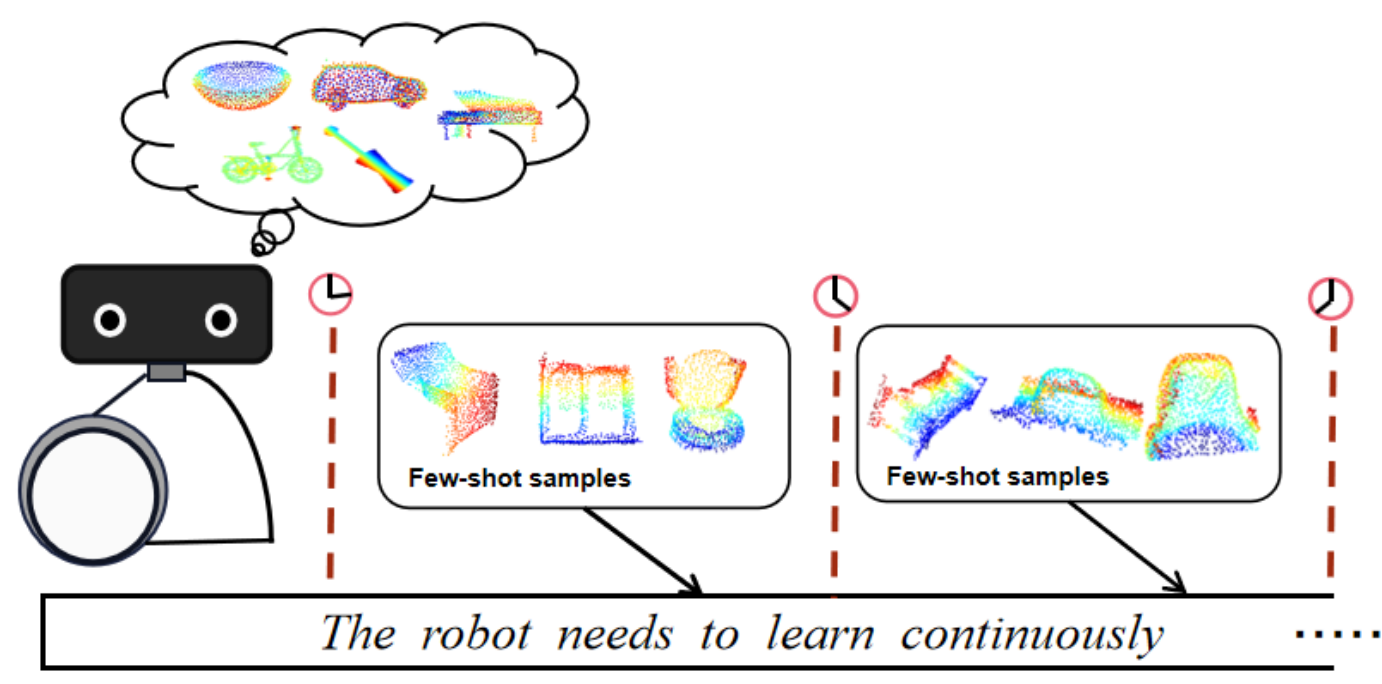
\includegraphics[width=0.82\linewidth,height=0.42\textheight,keepaspectratio]{figures/robot.png}
\end{figure}

机器人最初在合成三维数据上训练，部署后面对真实世界的点云扫描，需要不断学习新物体。在实验室里，我们可以用大量合成的 3D 模型训练它，比如从 ModelNet、ShapeNet 这样的数据中学习。但机器人真正部署到现实世界后，看到的却是另一番景象：真实物体的点云有噪声；物体可能被遮挡；扫描质量不稳定

不能把所有遗忘都看成同一种问题。遗忘分成两部分：

\begin{itemize}
  \item Base Class Forgetting：学习新类别时，原来的基础类别识别能力受到影响。
  \item Incremental Class Forgetting：随着后续增量学习，之前学过的新类别也可能被遗忘。
\end{itemize}

先识别来自哪个域，再决定交给哪个模型。对于基础类别，最重要的是不要破坏原来已经学好的模型。对于新增类别，模型又必须具备适应真实数据域的能力，并且在后续学习中保留这些知识。如果用同一个模型不断更新，就很难同时兼顾这两个目标。在这个 CrossDomain FSCIL 的工作中，我们把 OOD 检测从一个独立的检测任务，变成了持续学习系统中的一个路由机制：先判断样本是否属于基础分布，再决定调用哪一套知识。

\subsubsection*{第一步：判断是基础类别还是新增类别}

基础模型进行 ID / OOD 判断：判断是否属于原来的基础数据分布

测试时，先由基础模型判断样本是否属于基础分布：

\begin{itemize}
  \item 如果是，交给基础模型分类；
  \item 如果不是，则交给新类别模块分类。
\end{itemize}

\subsubsection*{第二步：新增类别做常规的增量学习}

虽然基础模型被冻结了，但新类别模块自己也可能遗忘，就按常规的同数据域下的类别增量学习去做。

实验也围绕这个场景展开，包括：

\begin{itemize}
  \item ModelNet $\rightarrow$ ScanObjectNN
  \item ShapeNet $\rightarrow$ CO3D
  \item ShapeNet $\rightarrow$ ScanObjectNN
\end{itemize}

而且采用 DGCNN 和 PointCLIP 等不同骨干进行实验，都验证了有效性。

总而言之，当新类别不仅是新的，而且来自一个不同的数据域时，这个 Cross-Domain FSCIL 的工作探讨了如何既保护原来的模型，又让新模型适应新的环境。当然，通常我们还是要将数据域的变化（协变量偏移）与标签域的变化（语义偏移）拆开。

\paragraph{相关工作}

\begin{itemize}
  \item Yuwen Tan, Xiang Xiang. Cross-Domain Few-ShotIncremental Learningfor Point-Cloud Recognition. In WACV, 2024.
\end{itemize}

\section{FADG：从频域信息到跨域泛化}

通常我们还是要将数据域的变化（协变量偏移）与标签域的变化（语义偏移）拆开。即使类别没有改变，原有模型也可能因为特征表示与当前环境不再匹配，而出现性能下降。这引出了一个不同于类别增量学习的问题：当模型已经部署、无法持续获得人工标注数据时，能否利用运行过程中不断到来的测试样本，主动调整模型，使其适应当前的数据分布？这一问题可以被归为领域泛化（Domain Generalization, DG）与测试时自适应（Test-Time Adaptation, TTA）一类问题——如果说类别增量学习关注的是模型如何适应语义知识的扩展，那么测试时自适应关注的则是模型如何适应部署环境中的数据分布变化。两者面对的变化类型不同，但背后有一个共同的问题：模型不能仅仅依赖训练阶段形成的固定知识，而需要具备在开放环境中持续调整自身的能力。

不同数据域的差异，会反映在频率成分上。假设同一辆汽车，分别在白天、夜晚、雨天和不同摄像头下拍摄。它的语义没有变化，但图像外观发生了变化：

\begin{itemize}
  \item 光照变化，会改变图像整体亮度和缓慢变化的结构信息。
  \item 不同成像设备，会带来不同的纹理、锐度和成像响应。
  \item 雨雪、模糊、噪声，会改变图像的局部细节和高频成分。
  \item 不同风格，也会改变图像的频率统计特征。
\end{itemize}

这些变化会反映在图像的频谱中。因此，频域提供了一种观察数据域差异的不同视角。原本在空间域中混合在一起的内容、风格、纹理和噪声，在频率分解之后，可以得到不同程度的区分。当然，频率不天然等于域不变信息。高频不一定代表语义，低频也不一定代表背景。不同频率成分都可能包含语义信息，也都可能受到域变化影响。

为什么这能够帮助模型适应？第一，分析分布变化。传统模型直接从图像中学习特征，但不一定清楚自己依赖了哪些频率信息。频域分解让我们可以进一步分析：模型究竟依赖哪些频率范围？这些信息在不同数据域之间是否稳定？第二，主动构造新的训练样本。不是简单地把高频信息作为额外输入，而是把不同数据域、相同语义类别的低频和高频成分重新组合。例如： A 域有汽车的低频信息， B 域有汽车的高频信息，于是可以将它们组合起来，构造新的训练样本。这样模型就不能只依赖某个特定域的完整视觉外观，而需要学习不同频率信息与类别语义之间的联系。第三，扩大模型能够利用的频率范围。让不同层级的子模型进行特征对齐，使较小的子模型也能获得较宽的频率感知能力。

\section{DEM：重新审视熵最小化——测试时适应}

在《FADG：从频域信息到跨域泛化》中，我们已经探究了如何在训练阶段增强模型面对未知数据域的泛化能力。但是，如果模型已经部署，新的数据分布已经出现，我们能不能让模型利用这些无标注的测试数据，主动调整自己？这就从 Domain Generalization（DG）转向 Test-Time Adaptation（TTA）。但首先，我们得思考一个问题：让模型的预测越来越确定，是否真的意味着模型适应得越来越好？

为什么需要测试时适应？在传统的机器学习流程中，模型训练和模型部署通常是两个相互分离的阶段。训练阶段，模型利用带有标签的数据学习输入与类别之间的关系；部署阶段，模型则直接对新的输入进行预测。这样的流程隐含了一个重要假设：训练数据和测试数据来自相同或相近的分布。然而，在开放环境中，这一假设往往难以成立。模型可能在晴天采集的图像上训练，却需要在雨天、夜间或不同摄像头采集的图像上工作。虽然物体的语义类别没有发生变化，但图像的外观和统计特征已经发生了改变。模型在训练阶段学到的决策边界，因而可能不再适合新的数据分布。一种自然的想法是：既然测试环境已经发生变化，为什么不让模型在测试阶段继续学习，利用当前环境中的数据调整自身？这就是测试时适应（Test-Time Adaptation，TTA）的基本思想。与传统训练不同，TTA 通常无法获得测试样本的真实标签，因此需要利用无标注数据构造自监督信号，引导模型进行调整。因此， TTA 的主要关注点一般是：如何利用无标注测试数据，让模型逐渐适应新的数据分布？

传统熵最小化有什么问题？一种广泛采用的方法是熵最小化（Entropy Minimization）。它的直觉很简单：如果模型已经适应了当前的测试环境，那么面对测试样本时，就应该能够给出更加确定的预测。因此，可以通过最小化预测概率分布的熵，让模型的预测逐渐变得更加集中。假设模型看到一张新的测试图片，输出：

\begin{itemize}
  \item 汽车：0.45
  \item 卡车：0.35
  \item 公交车：0.20
\end{itemize}

熵最小化希望模型通过测试时更新，让预测更加确定，例如变成：

\begin{itemize}
  \item 汽车：0.80
  \item 卡车：0.15
  \item 公交车：0.05
\end{itemize}

这样做似乎很合理：模型逐渐形成更加明确的决策边界，适应新的测试数据。但是，传统熵最小化存在两个内在问题。问题一：Reward Collapse（奖励塌缩）。直觉上，模型对一个样本越有把握，这个样本的预测结果就越值得信任。但传统熵最小化的梯度存在一个现象：当预测概率接近 1 时，样本对优化的贡献反而趋近于零。也就是说，一个已经被模型非常确定地识别出来的样本，反而无法继续提供足够的优化信号。问题二：Easy-Class Bias（容易类别偏置）。模型可能更容易识别某些类别，于是这些类别在测试时不断获得更高的预测概率。熵最小化进一步强化这些预测，导致模型越来越倾向于把样本分配给少数容易识别的类别。例如，模型在新环境中本来就容易把一些车辆识别成汽车，经过持续的熵最小化后，可能越来越多的样本都被归为汽车。这就产生了类别预测分布与真实类别分布之间的偏离。尤其在动态环境或类别不平衡的情况下，这个问题更加明显。

DEM 如何改进？有一次做信息来源的拆解——把熵最小化拆开来看：

\[
H(\mathbf{z})=\underbrace{-\sum_i p_i(\mathbf{z})\,z_i}_{\mathrm{CADF}}+\underbrace{\log\sum_i e^{z_i}}_{\mathrm{GMC}}
\]

这里的 $\mathbf{z}$ 是模型输出的 logits，$p_i$ 是 Softmax 后的类别概率。这两个部分实际上发挥着相反的作用。CADF（Cluster Aggregation Driving Factor）起推动作用，鼓励模型提高已有高概率类别的 logit，让预测分布更加集中，形成更明确的类别判断；GMC（Gradient Mitigation Calibrator）起校准作用，对高概率类别施加一定惩罚，抑制 logit 过度增长，避免模型过度偏向容易类别。熵最小化并不只是简单地让模型变得更加自信，它实际上包含了推动类别聚合和抑制过度自信的两种力量。传统方法将它们耦合在一个目标函数里，反而限制了两种力量各自发挥作用。

\begin{itemize}
  \item 针对 Reward Collapse：对 CADF 的 reward 进行归一化，增强高置信度样本在优化中
\end{itemize}

的贡献。

\begin{itemize}
  \item 针对 Easy-Class Bias：用 Marginal Entropy Calibrator（MEC）替代 GMC，通过动态估
\end{itemize}

计类别预测的边缘分布，抑制容易类别对模型的过度主导。

最终形成 AdaDEM（Adaptive Decoupled Entropy Minimization）。不需要预先知道目标域的类别先验分布，也不需要额外调节 DEM 中的温度和权重超参数。

\begin{figure}[H]\centering
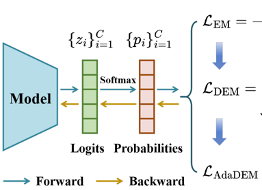
\includegraphics[width=0.82\linewidth,height=0.42\textheight,keepaspectratio]{figures/dem.png}
\caption*{熵最小化被解耦为两部分}
\end{figure}

实验方面，TTA 提升 8.4 个百分点和学习率容忍范围扩大 10 倍。DEM 并不只针对 TTA，还验证了半监督学习、无监督域适应和强化学习等任务。DEM 首先在 ImageNet-C 及ImageNet 的多个分布偏移基准上验证了方法的有效性。在 ViT-B/16 上，AdaDEM 相比传统熵最小化方法 Tent，在单域测试时适应和持续测试时适应任务中分别提升了 8.4 和 4.6 个百分点。同时，它对学习率的容忍范围扩大了约 10 倍，降低了测试时适应对超参数选择的敏感性。进一步地，将 AdaDEM 应用于 ETA、EATA、SAR 等不同测试时适应方法，并在CIFAR-10、CIFAR-100、STL-10、EuroSat 等六个半监督学习基准上进行了验证。在 EuroSat上，相比传统熵最小化，准确率提升了 7.2 个百分点。此外，还将其扩展到无监督域适应、长尾分类和强化学习任务。

以 ViT-B/16 为例：

\begin{table}[H]\centering
\caption*{ViT-B/16}
\begin{tabular}{lll}\toprule
\textbf{方法} & \textbf{单域 TTA} & \textbf{持续 TTA} \\ \midrule
No Adapt & 38.8\% & 38.8\% \\
Tent（传统熵最小化） & 53.1\% & 58.6\% \\
DEM* & 56.0\% & 64.1\% \\
AdaDEM & 61.5\% & 63.2\% \\
AdaDEM 相对 Tent & +8.4 & +4.6 \\
\bottomrule\end{tabular}
\end{table}

CLIP ViT-B/16 上：

\begin{table}[H]\centering
\caption*{CLIP ViT-B/16}
\begin{tabular}{lll}\toprule
\textbf{基础方法} & \textbf{单域 TTA 提升} & \textbf{持续 TTA 提升} \\ \midrule
Tent + AdaDEM & +8.4 & +4.6 \\
ETA + AdaDEM & +1.7 & +1.9 \\
EATA + AdaDEM & +3.1 & +1.5 \\
SAR + AdaDEM & +11.5 & +6.0 \\
\bottomrule\end{tabular}
\end{table}

\begin{table}[H]\centering
\caption*{半监督学习基准}
\begin{tabular}{llll}\toprule
\textbf{数据集} & \textbf{传统熵最小化} & \textbf{AdaDEM} & \textbf{提升} \\ \midrule
CIFAR-10 & 96.4 & 97.2 & +0.8 \\
CIFAR-100 & 72.6 & 75.8 & +3.2 \\
STL-10 & 82.4 & 84.8 & +2.4 \\
EuroSat & 76.5 & 83.7 & +7.2 \\
TissueMNIST & 47.3 & 49.3 & +2.0 \\
Semi-Aves & 59.9 & 61.0 & +1.1 \\
\bottomrule\end{tabular}
\end{table}

这些结果表明，DEM 不仅能够改善特定测试时适应方法的性能，也展示了其作为一种通用优化机制，在不同不完美监督学习任务中的应用潜力。在 TTA 实验中，AdaDEM 不仅用于单一目标域，也用于连续变化的目标域。

动态测试时自适应

总而言之，预测变得更加确定，并不意味着预测一定更加正确。如果模型最初就判断错误，熵最小化可能进一步强化这个错误判断。即使模型的预测已经非常确定，它也未必真正学到了适合新环境的知识。因此，熵最小化虽然提供了一种简单有效的测试时学习信号，却也可能带来新的优化问题。DEM 正是从这里出发，重新分析熵最小化的优化机制，并尝试回答更根本的问题：如何让模型在测试阶段不仅变得更加确定，而且能够更加可靠地适应新的数据分布？当我们利用模型自己的预测结果来指导模型更新时，这些自监督信号本身可靠吗？它们会不会在优化过程中产生偏差？

\paragraph{相关工作}

\begin{itemize}
  \item Jing Ma, Hanlin Li, Xiang Xiang*: Decoupled Entropy Minimization. In NeurIPS, 2025.
\end{itemize}

\section{PTTA：从样本筛选到样本净化}

在《DEM：重新审视熵最小化——测试时适应》中，模型需要利用无标注的测试数据不断调整自身。然而，并不是所有测试样本都能够为模型提供有益的学习信号。一些样本可能由于分布偏移而具有较高的不确定性，如果直接用于模型更新，反而可能破坏优化过程的稳定性。

因此，已有研究开始关注测试样本的筛选：识别有益样本，并过滤掉可能产生负面影响的样本。但这种做法也带来了新的问题——测试数据本来就有限，直接丢弃一部分样本意味着浪费其中可能仍然包含的有效信息。同时，样本筛选通常依赖预设阈值，阈值的微小变化也可能导致模型性能出现明显波动。

从样本选择到样本净化。传统 TTA 通常利用无标注测试样本进行自监督优化，例如通过熵最小化，让模型在测试数据上继续调整参数。但并不是所有测试样本都对模型有帮助。在分布偏移条件下，一些样本可能具有较高的不确定性，甚至产生错误的优化方向。例如，一个在晴天道路图像上训练的模型，部署到雨天环境后，可以利用雨天采集的图像进行适应。但这里有一个问题：测试数据虽然都来自真实环境，却不一定都能帮助模型学习。如果模型直接利用这些样本进行更新，可能放大已有偏差，破坏适应过程的稳定性。因此，已有方法通常会设计样本选择机制：识别有益样本，过滤掉可能有害的样本。但这带来一个问题：测试数据本来就有限，过滤样本意味着浪费其中可能仍然包含的有效信息。PTTA 换了一个思路：不再满足于识别和丢弃有害样本，而是尝试将它们转化为可以利用的样本。既然有害样本不适合直接用于模型适应，能不能找到一个对模型优化产生相反影响的良性样本，把两者组合起来？假设有一张测试图片 A，它会让模型沿着某个方向更新参数，而这个方向可能是不利的；我们再找一张良性图片 B，它对优化目标产生的影响方向与 A 相反；如果把 A 和 B 混合起来，可能就能减弱 A 原本带来的不良影响。

\begin{figure}[H]\centering
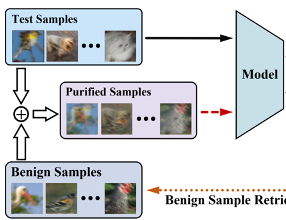
\includegraphics[width=0.82\linewidth,height=0.42\textheight,keepaspectratio]{figures/ptta.png}
\caption*{为什么不把有害样本变成有用样本？}
\end{figure}

如何衡量样本对优化的影响？模型训练时会根据损失函数的梯度调整参数。PTTA 进一步考虑：能不能直接观察一张输入图片对优化目标产生的影响？以熵最小化作为例子，对于一张测试图片 $x$，计算熵损失相对于输入的梯度：

这个梯度描述了：如果希望降低这张图片对应的预测熵，输入空间中的变化应该朝哪个方向进行。如果两张图片的梯度方向相近，说明它们对优化目标的影响比较相似；如果梯度方向相反，则说明它们可能产生相反的优化影响。据此定义 Saliency Distance：

\[
D_{sa}(x_i,x_j)=1-\mathrm{Cosine}(g_{x_i},g_{x_j})
\]

\noindent 距离越大，代表两张样本对应的梯度方向越不一致。我们比较了三种 Saliency Indicator：

\begin{itemize}
  \item Pixel-level：在原始图像空间计算梯度，保留空间细节，但容易受到无关像素影响。
  \item Feature-level：在特征空间计算梯度，利用网络提取的语义表征，减少无关像素干
\end{itemize}

扰。

\begin{itemize}
  \item Logit-level：在分类输出空间计算梯度，直接衡量样本对最终分类决策的影响。实
\end{itemize}

验发现，Logit-level 指标总体表现较好，而且计算开销更低。它可以直接利用模型输出计算，不需要额外对输入或特征反向传播。

Logit-level 指标总体表现较好，而且计算开销更低。它可以直接利用模型输出计算，不需要额外对输入或特征反向传播。这是在效率和效果之间作出的一个权衡。

到哪里寻找良性样本？有了 Saliency Indicator，接下来就是寻找与有害样本优化影响最不一致的良性样本。我们研究了三种检索方式：

\begin{table}[H]\centering
\begin{tabular}{lll}\toprule
\textbf{检索方式} & \textbf{良性样本来源} & \textbf{特点} \\ \midrule
ID Retrieval & 训练阶段的源域数据 & 使用固定的源域样本库 \\
OOD Retrieval & 历史测试阶段的良性样本 & 使用 FIFO 队列动态更新 \\
In-Batch Retrieval & 当前 mini-batch & 不需要额外的 memory bank \\
\bottomrule\end{tabular}
\end{table}

在持续 TTA 中，模型会逐渐适应目标域，但也可能遗忘原来的源域知识。因此，不仅要考虑从训练数据中寻找良性样本，也考虑把过去测试过程中筛选出的良性样本保存在memory bank 中，供后续使用。检索时，对每个有害样本，选择 Saliency Distance 最大的良性样本作为配对对象。这相当于在优化影响空间中，寻找一个最有可能与它形成互补的样本。

如何净化？找到配对样本后，可使用经典的 Mixup。假设有害样本为 $x_i$，检索到的良性样本为 $x_j^{*}$，对应的模型预测概率分别为 $\hat{y}_i$ 和 $\hat{y}_j^{*}$。组合后得到：

\[
x^{*}_{ij}=\lambda x_i+(1-\lambda)x_j^{*}
\]

对应的软标签为：

\[
\hat{y}^{*}_{ij}=\lambda\hat{y}_i+(1-\lambda)\hat{y}_j^{*}
\]

设置：

\[
\lambda=\frac{1}{K+1}
\]

其中 $K$ 是检索的良性样本数量。默认 $K=1$，因此两张图片各占一半。

随后，利用组合后的样本计算交叉熵形式的 Purification Loss：

\[
\mathcal{L}_{pur}=-\frac{1}{N}\sum_{i,j}\hat{y}^{*}_{ij}\log\sigma\bigl(f_\theta(x^{*}_{ij})\bigr)
\]

最后，把它加入原有 TTA 的优化目标：

\[
\mathcal{L}=\mathcal{L}_{TTA}+\alpha\,\mathcal{L}_{pur}
\]

因此，PTTA 不需要重新设计原有 TTA 算法的主体，只需要增加一个净化损失，就能作为一个 Plug-and-Play 模块使用。

实验覆盖四种 TTA 设置：

\[
\lambda=\frac{1}{K+1}
\]

\begin{itemize}
  \item Episodic TTA
  \item Single TTA
  \item Continual TTA
  \item Lifelong TTA
\end{itemize}

同时涉及图像分类、语义分割和对抗防御任务。

其中，比较重要的发现是：PTTA 并不是只对某一个 TTA 算法有效，而是可以与 ETA、DeYO、CPL、CoTTA、SoTTA、SAR、EATA 等方法结合。

例如，在 ImageNet-C 的 ViT-B/16 实验中：

\begin{table}[H]\centering
\caption*{ImageNet-C，ViT-B/16}
\begin{tabular}{lll}\toprule
\textbf{方法} & \textbf{Single TTA} & \textbf{Continual TTA} \\ \midrule
Tent & 51.3 & 14.2 \\
Tent + PTTA & 52.1 & 60.1 \\
SoTTA & 57.1 & 59.5 \\
SoTTA + PTTA & 58.1 & 61.3 \\
SAR & 56.7 & 60.0 \\
SAR + PTTA & 58.0 & 61.6 \\
\bottomrule\end{tabular}
\end{table}

这里尤其值得注意的是 Tent 在 Continual TTA 中的表现：加入 PTTA 后，从 14.2 提升到了60.1。这说明在持续适应中，处理不可靠测试样本对稳定性可能非常重要。在 Lifelong TTA中，论文还考察了连续十轮测试分布变化。以 ETA 为例，原始方法的平均准确率为 39.0\%，加入 PTTA 后达到 64.8\%。此外，我们还做了 Saliency Indicator、检索范围、Mixup 数量和损失权重等消融实验，验证方法设计的合理性。

总而言之，测试数据并不是简单地分成有用和无用两类。即使某些数据不能直接用于模型适应，也可能通过与其他数据建立互补关系，重新获得利用价值。首先，PTTA 从样本筛选转向样本利用——传统方法关注如何识别不可靠样本并把它们过滤掉。PTTA 则进一步考虑：这些样本虽然不适合直接用于适应，但是否还能通过与其他样本组合重新利用？其次，从样本自身的属性转向样本之间的关系。PTTA 并不只看一张图片的熵有多大，而是比较不同样本对优化目标的影响方向。它把样本之间的优化关系作为寻找互补样本的依据。再次，从单纯的数据过滤转向数据净化。它没有改变原有 TTA 的主体优化机制，而是在原有方法上增加一个净化过程，使更多测试数据能够参与适应。在更广泛的意义上，FADG、DEM、PTTA 的共同点，是在分布偏移条件下，挖掘和利用仍然有效的信息。它们的差异在于处理问题的层次不同：

\begin{enumerate}
  \item PTTA 关注数据质量：测试数据中可能存在有害样本，需要先判断哪些样本适合参
\end{enumerate}

与适应。

\begin{enumerate}
  \item DEM 关注优化机制：即使使用无标注测试数据，传统熵最小化也可能出现 Reward
\end{enumerate}

Collapse 和 Easy-Class Bias，需要重新设计优化信号。

\begin{enumerate}
  \item Frequency-Aware DG 关注特征表征：不同域的频率成分具有不同的信息，需要扩大
\end{enumerate}

模型能够有效感知和利用的频率范围。

从研究层次上说：PTTA 是数据质量优化，DEM 适应目标优化，FADG 是特征表征优化。相关工作：

\begin{itemize}
  \item Jing Ma, Hanlin Li, Xiang Xiang*: PTTA: Purifying Malacious Samples forTest-Time Model
\end{itemize}

Adaptation. In ICML, 2025.

\begin{figure}[H]\centering
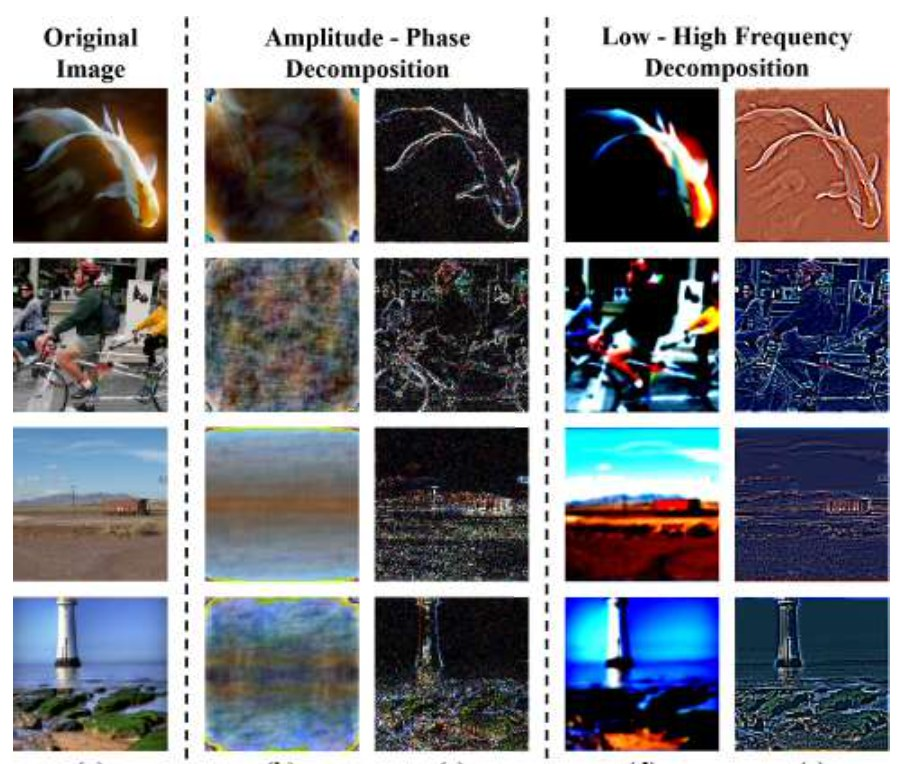
\includegraphics[width=0.82\linewidth,height=0.42\textheight,keepaspectratio]{figures/fadg.jpg}
\caption*{处理流程，以及与振幅—相位分解方法生成图像的对比}
\end{figure}

不同模型为什么具有不同的跨域泛化能力？DG 需要的不是简单的数据增强，而是主动构造不同频率成分之间的跨域组合，让模型学习更广泛的频率信息与语义类别之间的联系。不同模型对图像不同频率成分的感知能力并不相同，而且这种能力与模型的泛化能力存在关联。我们将模型在不同频率范围内仍能保持 90\% 测试准确率的频率区间，定义为它的Frequency-Aware Region。对输入图像施加不同强度的低通滤波，逐渐去除高频信息，然后观察模型的分类准确率如何变化：相同架构下，CLIP 预训练模型的 Frequency-Aware Region 通常比 ImageNet 预训练模型更宽。据此提出一个假设：泛化能力更强的模型，能够从更广泛的图像频率范围中提取与语义类别有关的信息。我们这种观察转化为训练策略，再进一步利用测试阶段的无标注数据改善预测。

不是简单地把高频信息加进训练数据。首先，对一张图像进行傅里叶变换，然后利用Gaussian Filter 将其分解为低频和高频部分：

\[
\begin{gathered}X_l=X\odot G \\ x_l=\mathrm{IDFT}(X_l) \\ x_h=x-x_l\end{gathered}
\]

其中：

\begin{itemize}
  \item $x_l$：低频图像，保留整体结构和缓慢变化的视觉信息。
  \item $x_h$：高频图像，保留边缘、纹理和细节等信息。
\end{itemize}

这里采用 Gaussian Filter，而不是直接用硬阈值截断频率。原因是硬截断可能破坏低频和高频之间的关联，导致合成图像质量下降。接下来，从同一个语义类别、不同数据域的两张图像中，取一张的低频部分和另一张的高频部分，再进行 Mixup。

具体为：

\[
\hat{x}=\lambda\,x_l^{m_1}+(1-\lambda)\,x_h^{m_2}
\]

其中：

也就是说，两张图像来自不同域，但属于相同类别。假设我们有一张真实照片中的汽车，以及一张卡通风格的汽车。我们希望模型不仅能够识别真实照片中的汽车，也能够从卡通风格图像的细节、轮廓等信息中学习有用的语义特征。通过低频与高频的跨域组合，模型可以接触到更多不同频率组成的图像，同时保持类别语义一致。还可以自适应地确定频率分界阈值，使低频与高频部分的频谱能量相等，这样生成的混合图像不容易出现明显失真。不同规模的模型具有不同的 Frequency-Aware Region？我们观察到：较大的模型通常具有更宽的频率感知范围，也具有更强的零样本泛化能力。那么，能不能让较小的模型学习较大模型的频率感知能力？我们将一个网络拆分成多个连续的 block，并在每个 block 后面增加一个轻量级分类器——利用较深层、更具泛化能力的表示，指导较浅层子模型学习更具域不变性的特征。

在多个域泛化基准上进行了验证，包括 PACS、VLCS、Office-Home、TerraIncognita、DomainNet，以及 KITTI 目标检测。

ResNet-50 多源域泛化

\begin{table}[H]\centering
\caption*{ResNet-50 多源域泛化}
\begin{tabular}{ll}\toprule
\textbf{方法} & \textbf{平均准确率} \\ \midrule
ERM & 63.3\% \\
FBBT & 67.0\% \\
FBBT + FEI（CLP） & 68.8\% \\
\bottomrule\end{tabular}
\end{table}

Office-Home，ResNet-18

\begin{table}[H]\centering
\caption*{Office-Home，ResNet-18}
\begin{tabular}{ll}\toprule
\textbf{方法} & \textbf{平均准确率} \\ \midrule
ERM & 60.6\% \\
FBBT & 68.0\% \\
FBBT + FEI（CLP） & 70.7\% \\
\bottomrule\end{tabular}
\end{table}

PACS，多种网络架构

\begin{table}[H]\centering
\caption*{PACS，多种网络架构}
\begin{tabular}{llll}\toprule
\textbf{Backbone} & \textbf{ERM} & \textbf{FBBT} & \textbf{FBBT + CLP} \\ \midrule
AlexNet & 71.5\% & 77.2\% & 80.3\% \\
ResNet-18 & 80.0\% & 87.3\% & 89.0\% \\
ResNet-50 & 83.3\% & 89.2\% & 90.5\% \\
\bottomrule\end{tabular}
\end{table}

这些结果说明两件事：

\begin{enumerate}
  \item FBBT 在训练阶段扩大频率感知范围，已经能显著改善域泛化。
  \item CLP 在测试阶段进一步利用目标域内部的相似关系，还能带来额外收益。
\end{enumerate}

论文还在 KITTI 上验证了雾、雨、雪等天气变化下的目标检测性能，并将方法应用到 CLIP和其他已有 DG 方法中。

总而言之，我们从图像频率的角度重新审视模型的泛化能力。通过分析不同模型对图像频率成分的感知范围，我们发现，泛化能力更强的模型通常具有更宽的频率感知区域。基于这一观察，我们进一步提出频率分解与混合、层级特征对齐等方法，扩大模型对不同频率信息的感知能力，并在测试阶段利用不同层级的特征进行集成和标签传播。

这条路径的核心是：在环境变化真正发生之前，尽可能让模型具备面对未知环境的能力。但训练阶段的准备并不能解决所有问题。真实环境中的数据分布可能持续变化，模型仍然可能遇到训练阶段无法预料的情况。这时，另一种思路就变得重要：能否在模型部署之后，利用不断到来的无标注测试数据，主动调整模型？在测试时自适应（Test-Time Adaptation）中，我们开始研究模型如何在缺少人工标注的情况下，利用自身的预测结果适应新的数据分布。

\paragraph{相关工作}

\begin{itemize}
  \item Xiang Xiang*, Jing Ma, Hanlin Li. Frequency-Aware Domain Generalization. IEEE Trans. Image Processing, 2026.
\end{itemize}
